\section{Architektur und Designentscheide}
\subsection{Modell(e) und Sichten}

\subsubsection{Klassenüberischt}
Die Klasse SimpleLoggerSetup implementiert das LoggerSetup-Interface und ist aufgrund dessen in der Lage ein Logger vom Typ des Logger-Interfaces zu konfigurieren. Der Logger wird durch eine Factory-Methode erstellt und an den Aufrufer zurückgeliefert. Der Logger selbst bietet nun die Möglichkeit die definierten Level zu loggen und besitzt eine Referenz auf den sogenannten Client-Socket, welcher durch den LoggerSetup erstellt wurde. Dieser Client-Socket stellt eine Verbindung über TCP/IP zum Server-Socket her. Somit ist es dem Logger möglich Log-Einträge an einen Server zu übermitteln. Der Logger-Server wird durch das Event Listener-Pattern über neue Log-Einträge informiert und kann diese verarbeiten. Zu guter Letzt werden die Log-Einträge über das StringPersistor-Interface und die StrinPersistorFile-Klasse in eine dafür vorgesehene Datei geschrieben.

\begin{figure}[H]
	\centering
	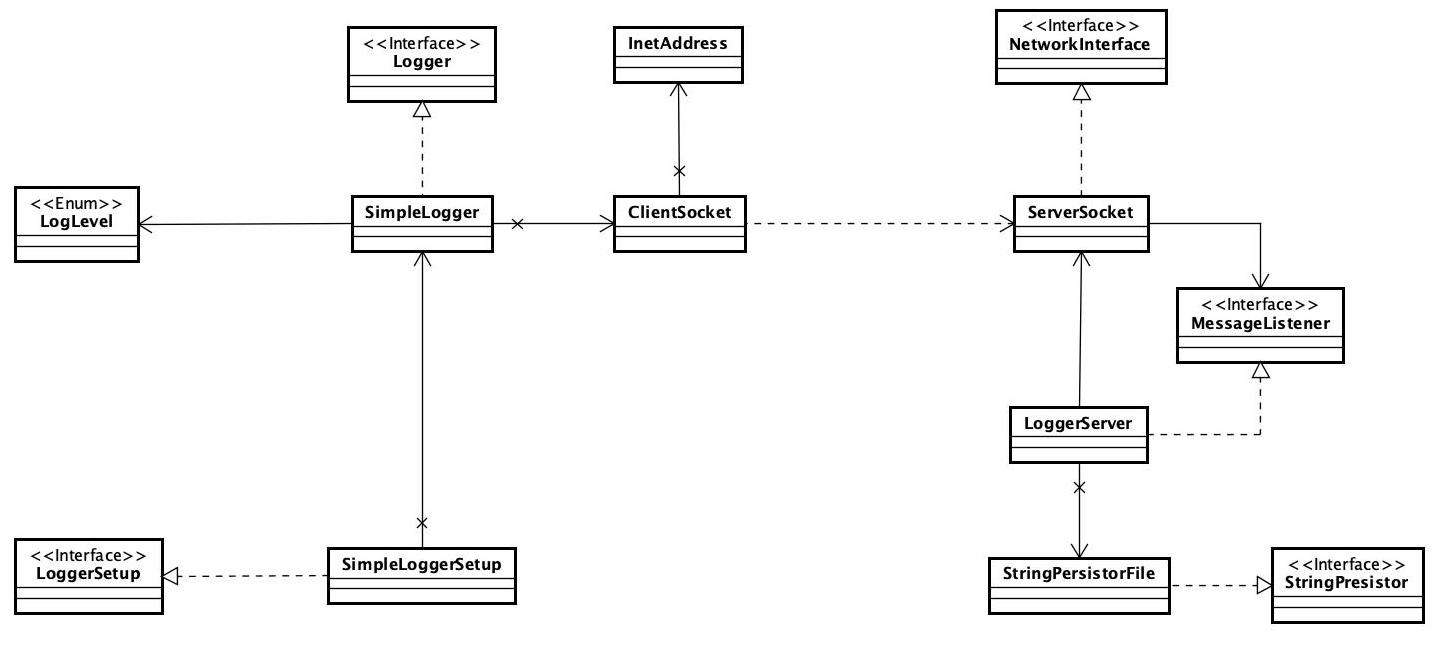
\includegraphics[width=\textwidth]{2_Architektur/Bilder/classOverview.png}
	\caption{Klassendiagram}
	\label{fig:classdiagram }
\end{figure}

\newpage
\subsubsection{LoggerSetup}
Die Klasse LoggerFactory implementiert das zur Verfügung gestellte Interface LoggerSetup. Aufgrund dessen besitz die Klasse alle Methoden, um als LoggerSetup fungieren zu können. In der öffentlichen Methode createClientSocket() wird ein ClientSocket instanziiert, welcher eine Verbindung zum LoggerServer über die im LoggerFactory angegebene IP und Port aufbaut. Die LoggerSetupFactory Klasse wird dazu verwendet, das LoggerSetup mittels createLoggerSetup() über einen String und später auch über eine Konfigurationsdatei zu erstellen. 

\begin{figure}[H]
	\centering
	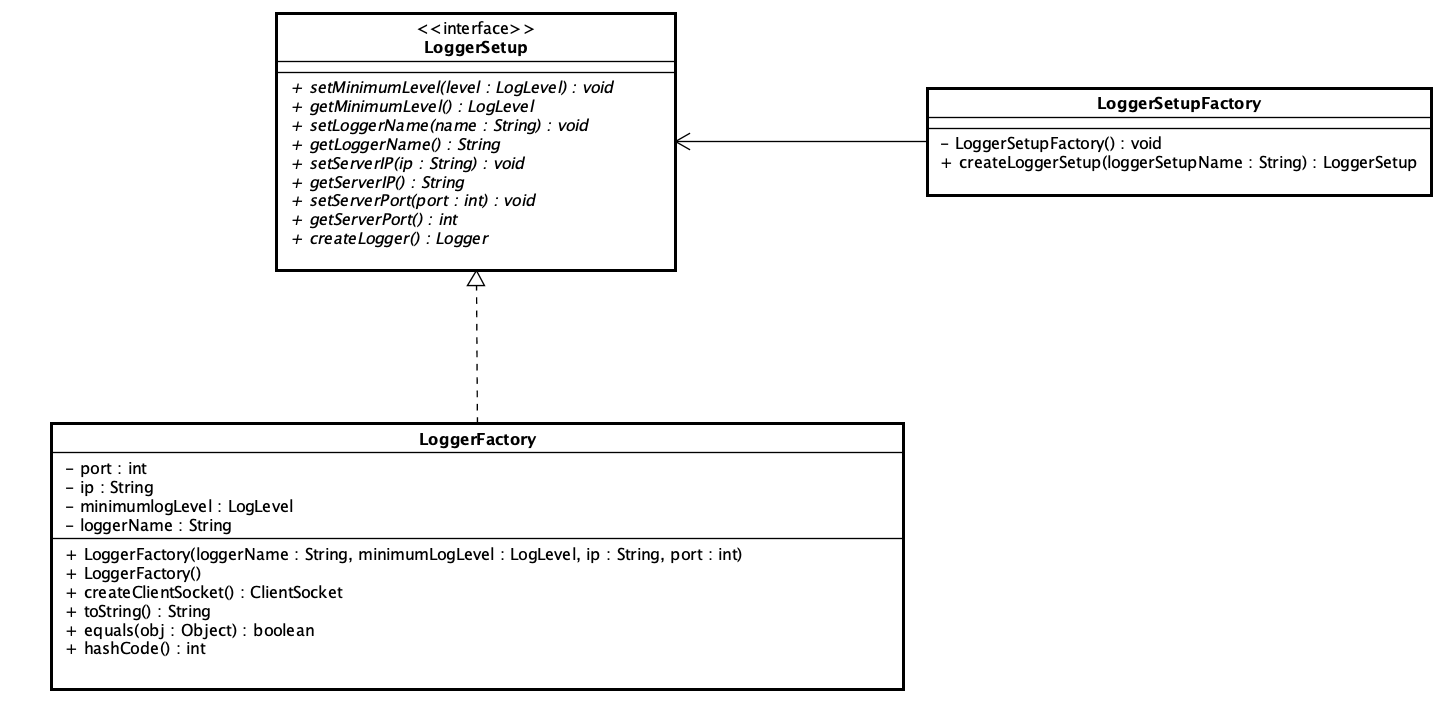
\includegraphics[width=\textwidth]{2_Architektur/Bilder/loggerFactory.png}
	\caption{LoggerFactory Klassendiagram}
	\label{fig:LoggerFactory Klassendiagramm}
\end{figure}

\newpage
\subsubsection{Logger}
Die Klasse BaseLogger implementiert das zur Verfügung gestellte Interface Logger. Aufgrund dessen besitzt die Klasse alle Methoden, um als Logger fungieren zu können. In der privaten Methode maybeLog() wird eine Überprüfung durchgeführt, welche mit Hilfe des minimalen Log-Levels entscheidet, ob eine Nachricht geloggt werden soll oder nicht. Soll eine Nachricht geloggt werden, wird in der Methode createLogMessage() ein Objekt der Klasse LogMessage instantiert und alle notwendigen Informationen diesem Objekt beigefügt. Schliesslich wird die Nachricht seralisiert und dem ClientSocket zum Senden übergeben. Aufgrund der Seralisierung implementiert die LogMessage-Klasse das Serializable-Interface.

\begin{figure}[H]
	\centering
	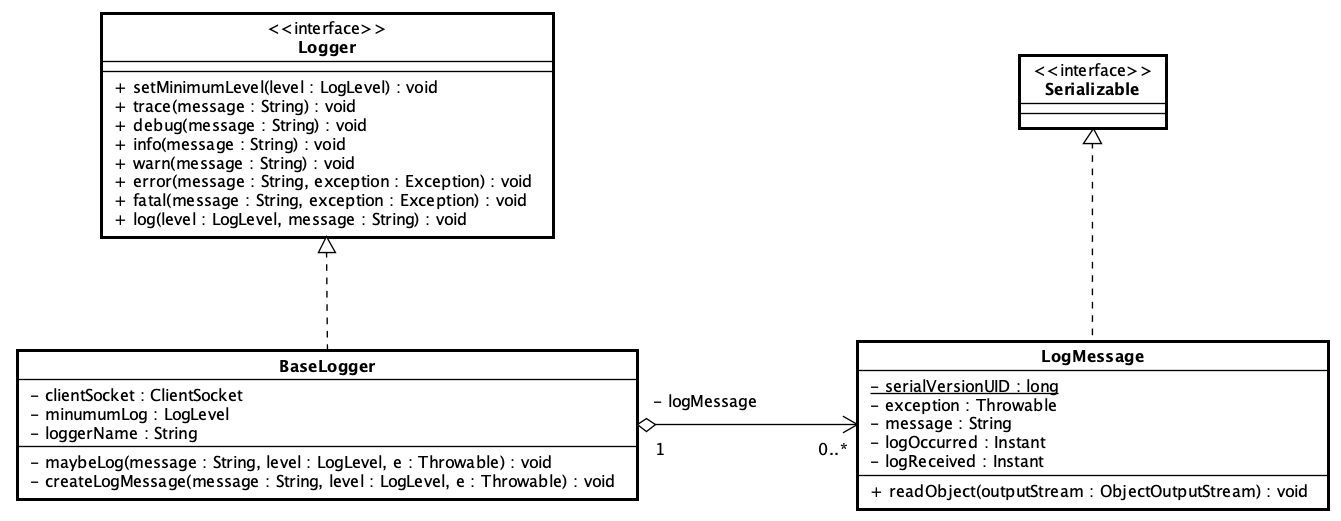
\includegraphics[width=\textwidth]{2_Architektur/Bilder/loggerClasses.png}
	\caption{Logger Klassendiagramm}
	\label{fig:Logger Klassendiagramm}
\end{figure}

\newpage
\subsubsection{Logger-Server}
Der Logger-Server besteht aus zwei Klassen, dem Logger-Server und dem LoggerServerSocket. Der Logger-Server ist lediglich für die Weiterleitung der LogMessages an den StringPersistor zuständig und implementiert zusätzlich die main-Methode, um den Startpunkt des Servers zu definieren. 
Die Klasse LoggerServerSocket implementiert die benötigte Logik zur Entgegennahme der an den Server gesendeten Log-Messages. Die einzelnen Messages werden in einzelnen Threads parallel abgearbeitet und an den LoggerServer übergeben. 

\begin{figure}[H]
	\centering
	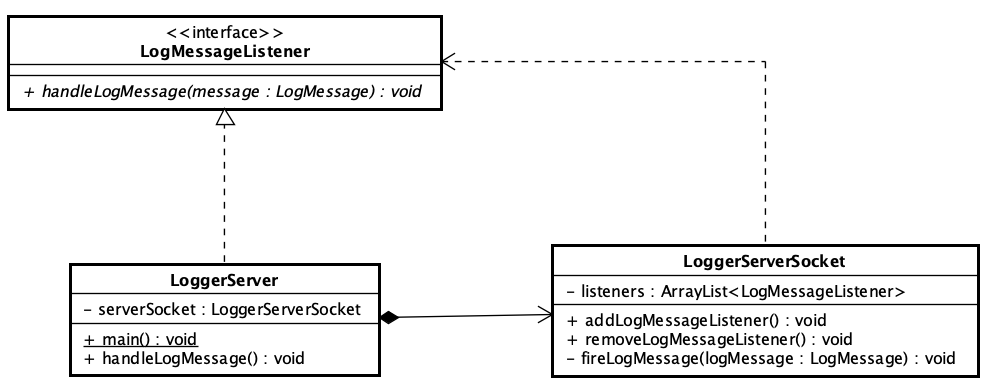
\includegraphics[width=\textwidth]{2_Architektur/Bilder/loggerServer.png}
	\caption{Logger-Server Klassendiagramm}
	\label{fig:Logger-Server Klassendiagramm}
\end{figure}

\newpage
\subsubsection{StringPersistor}
Die Klasse StringPersistorFile implementiert das zur Verfügung gestellte Interface StringPersistor. Aufgrund dessen besitzt die Klasse alle Methoden, um als StringPersistor fungieren zu können.
Mit der Methode save() welcher über den Adapter zur Verfügung steht wird die LogMessage in einen String umgewandelt und mit dem entsprechenden Zeitstempel ins File geschrieben. Die Messages werden über einen printWriter in das File geschrieben. Über die Methode setFile() wird das Textfile erstellt und über die Methode get() können diese Files wieder zurückgegeben werden. 

\begin{figure}[H]
	\centering
	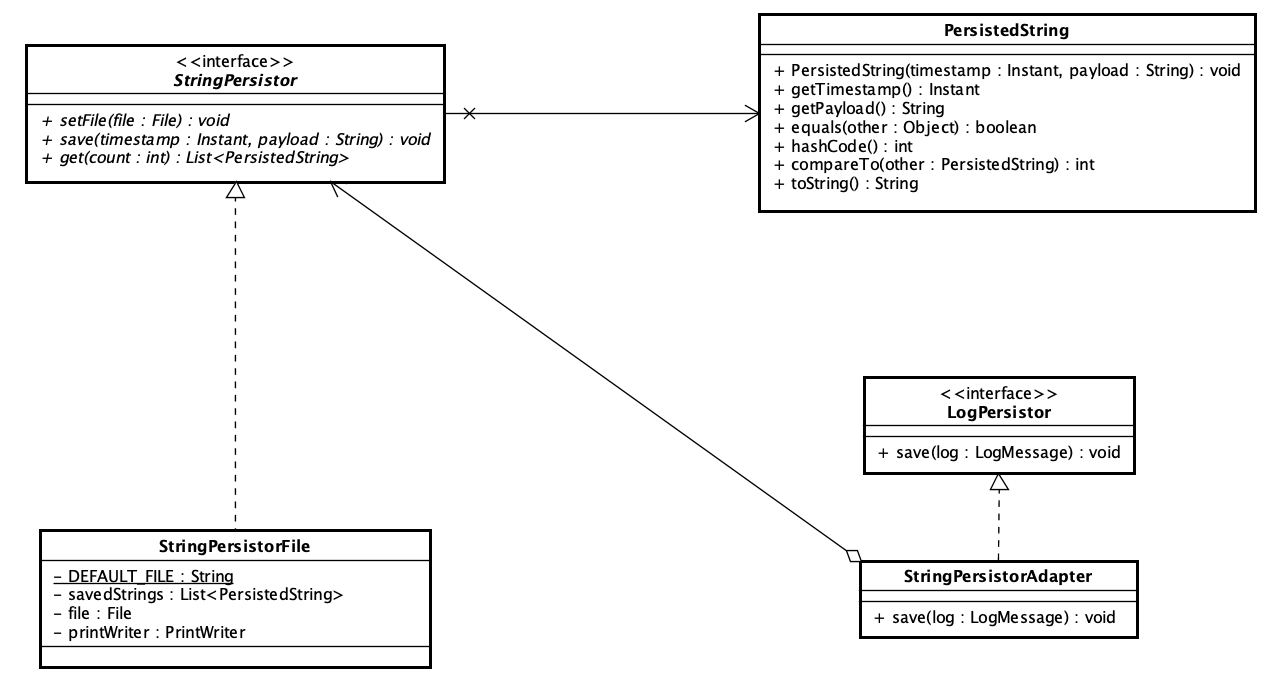
\includegraphics[width=\textwidth]{2_Architektur/Bilder/stringPersistor.png}
	\caption{StringPersistor Klassendiagramm}
	\label{fig:StringPersistor Klassendiagramm}
\end{figure}

\newpage
\subsection{Daten (Mengengerüst \& Strukturen)}
Zur Festhaltung der Daten werden sogenannte LogMessages generiert. Wie dies genau geschieht ist in der Abbildung \ref{fig:Logger Klassendiagramm} ersichtlich.

\subsubsection{Mengengerüst}
Da es sich um eine Logger Komponente handelt, die an diversen Stellen eingesetzt wird, kann das Mengengerüst nicht klar definiert werden.

\subsubsection{Strukturen}
Die Struktur der LogMessages, welche auch über den Adapter in Textfiles gespeichert werden sieht wie folgt aus:
\begin{itemize}
	\item LogLevel, definiert welches Level dem Log entspricht:
	\begin{itemize}
		\item Off
		\item Trace
		\item Debug
		\item Info
		\item Warn
		\item Error
		\item Fatal
	\end{itemize}
	\item Message, gibt mittels eines Strings eine Meldung mit.
	\item LogOccured, gibt den Zeitstempel mit, wann das Log erstellt wurde.
	\item LogReceived, gibt den Zeitstempel mit, wann das Log auf dem LoggerServer empfangen wurde.
\end{itemize}

\newpage
\subsection{Entwurfsentscheide}
\subsubsection{Event / Listener Pattern}
Das Event/Listener-Pattern wurde in Bezug auf den Logger-Server verwendet. Da der Logger-Server einen LoggerServerSocket beinhaltet, dieser jedoch dem Logger-Server die neuen Messages mitteilen muss, entsteht eine zirkuläre Beziehung zwischen diesen beiden Objekten. 
Um diese zirkuläre Beziehung aufzulösen und dadurch die Kopplung zu minimieren wird das Event/Listener-Pattern eingesetzt. Dadurch kommuniziert der LoggerServerSocket nur noch über das definierte Interface mit dem LoggerServer. Die komplette LoggerServer-Komponente ist unter Abbilung \ref{fig:Logger-Server Klassendiagramm} ersichtlich.
\begin{figure}[H]
	\centering
	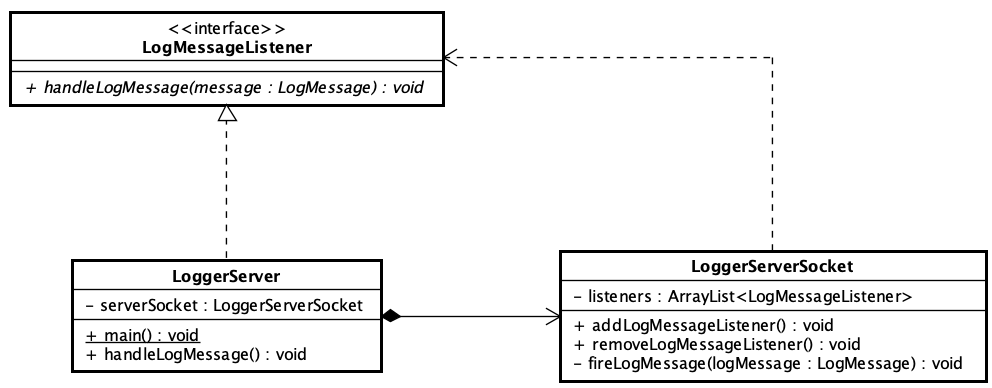
\includegraphics[width=\textwidth]{2_Architektur/Bilder/loggerServer_EventListener.png}
	\caption{Event / Listener Pattern}
	\label{fig:Event / Listener Pattern}
\end{figure}

\subsubsection{Adapterpattern}
Das Adapter Entwurfsmuster ist auf die String Persistor Schnittstelle angewendet. Dadurch kann die Komplexität der String Adapter Schnittstelle auf die benötigten Funktionen reduziert werden. Desweitern ist die neue Log Persistor Schnittstelle anwenderfreundlicher im Kontext des Loggers. Die LogPersistor Schnittstelle wird in Abbildung \ref{fig:Adapterpattern} dargestellt.
\begin{figure}[H]
	\centering
	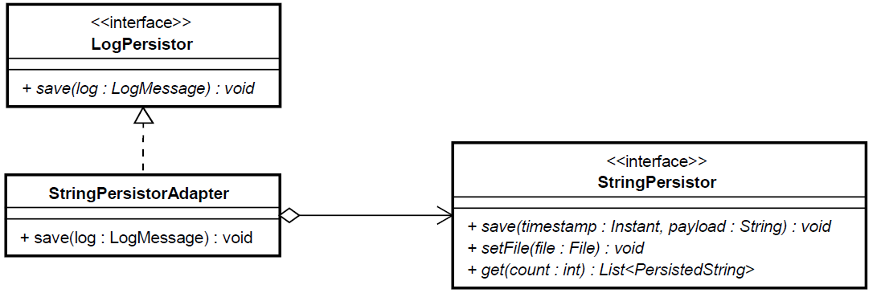
\includegraphics[width=\textwidth]{2_Architektur/Bilder/adapterpattern.png}
	\caption{Adapterpattern}
	\label{fig:Adapterpatternn}
\end{figure}

